% ============================================
% CHƯƠNG 3: THIẾT KẾ ỨNG DỤNG
% ============================================

\section{Thiết kế ứng dụng}

% ------------------------------------------
\subsection{Thiết kế cơ sở dữ liệu}

Hệ thống sử dụng cơ sở dữ liệu MySQL/MariaDB. Schema được định nghĩa trong file \texttt{db/sachhay\_db.sql} và đang được sử dụng trực tiếp trong ứng dụng.

\textbf{Các bảng chính:}

\begin{table}[H]
\centering
\begin{tabular}{|l|l|l|}
\hline
\textbf{Tên trường} & \textbf{Kiểu dữ liệu} & \textbf{Mô tả} \\
\hline
user\_id & INT (PK) & Khóa chính \\
password & VARCHAR(100) & Mật khẩu đã hash \\
fullname & VARCHAR(50) & Họ tên đầy đủ \\
email & VARCHAR(100) & Email người dùng \\
phone & VARCHAR(20) & Số điện thoại \\
role & VARCHAR(50) & Vai trò (customer/admin/staff) \\
created\_date & DATE & Ngày tạo tài khoản \\
\hline
\end{tabular}
\caption{Bảng users - Quản lý người dùng}
\label{tab:users}
\end{table}

\begin{table}[H]
\centering
\begin{tabular}{|l|l|l|}
\hline
\textbf{Tên trường} & \textbf{Kiểu dữ liệu} & \textbf{Mô tả} \\
\hline
product\_id & INT (PK) & Khóa chính \\
title & VARCHAR(255) & Tên sản phẩm \\
publisher & VARCHAR(100) & Nhà xuất bản \\
published\_date & DATE & Ngày xuất bản \\
description & TEXT & Mô tả chi tiết \\
pages & INT & Số trang \\
stock\_quantity & INT & Số lượng tồn kho \\
price & DECIMAL(12,2) & Giá bán \\
old\_price & DECIMAL(12,2) & Giá gốc \\
dimensions & VARCHAR(50) & Kích thước \\
\hline
\end{tabular}
\caption{Bảng product - Quản lý sản phẩm}
\label{tab:products}
\end{table}

\begin{table}[H]
\centering
\begin{tabular}{|l|l|l|}
\hline
\textbf{Tên trường} & \textbf{Kiểu dữ liệu} & \textbf{Mô tả} \\
\hline
order\_id & INT (PK) & ID đơn hàng \\
user\_id & INT (FK) & ID người dùng đặt hàng \\
recipient\_name & VARCHAR(255) & Tên người nhận \\
recipient\_phone & VARCHAR(20) & Số điện thoại người nhận \\
shipping\_address & TEXT & Địa chỉ giao hàng \\
payment\_method & VARCHAR(50) & COD/E-wallet/Credit Card \\
total\_amount & DECIMAL(10,2) & Tổng tiền đơn hàng \\
status & ENUM & pending/processing/shipped/completed/cancelled \\
created\_at & TIMESTAMP & Thời gian tạo đơn \\
\hline
\end{tabular}
\caption{Bảng orders - Quản lý đơn hàng}
\label{tab:orders}
\end{table}

\begin{table}[H]
\centering
\begin{tabular}{|l|l|l|}
\hline
\textbf{Tên trường} & \textbf{Kiểu dữ liệu} & \textbf{Mô tả} \\
\hline
order\_id & INT (PK) & ID đơn hàng \\
product\_id & INT (PK) & ID sản phẩm \\
quantity & INT & Số lượng \\
price & DECIMAL(10,2) & Giá tại thời điểm đặt \\
subtotal & DECIMAL(10,2) & Thành tiền \\
\hline
\end{tabular}
\caption{Bảng order\_product - Chi tiết sản phẩm trong đơn}
\label{tab:order_product}
\end{table}

\textbf{Các bảng liên quan khác:}
\begin{itemize}
    \item \texttt{category}, \texttt{category\_product}: danh mục và liên kết sản phẩm
    \item \texttt{product\_image}, \texttt{author\_of\_product}: hình ảnh và tác giả
    \item \texttt{cart\_items}: giỏ hàng của người dùng
    \item \texttt{wishlist}: sản phẩm yêu thích
    \item \texttt{user\_addresses}: địa chỉ giao hàng
    \item \texttt{news}, \texttt{comments}, \texttt{qa}, \texttt{contacts}: nội dung và tương tác
\end{itemize}

% ------------------------------------------
\subsection{Kiến trúc MVC tự xây dựng}

Dự án áp dụng mô hình MVC (Model-View-Controller) được xây dựng hoàn toàn từ đầu, không sử dụng framework có sẵn như Laravel hay Symfony. Điều này giúp hiểu sâu về cách thức hoạt động của pattern MVC.

\subsubsection{Luồng hoạt động MVC}

Luồng xử lý request được tổ chức theo các bước sau, giúp tách biệt rõ phần điều hướng, xử lý nghiệp vụ và hiển thị:
\begin{enumerate}
    \item Người dùng gửi request tới server (ví dụ: \texttt{/product/detail/1}).
    \item \texttt{public/index.php} là điểm vào (entry point), chuyển request vào \texttt{app/router.php}.
    \item \texttt{App.php} phân tích URL, xác định \texttt{controller}, \texttt{method} và \texttt{params}.
    \item Controller nhận request, kiểm tra dữ liệu đầu vào, gọi Model cần thiết.
    \item Model truy vấn DB (thông qua \texttt{DB.php}) và trả dữ liệu về Controller.
    \item Controller đóng gói dữ liệu và gọi View để render HTML.
    \item View trả về HTML và server gửi phản hồi cho trình duyệt.
\end{enumerate}

Trong các thao tác AJAX (giỏ hàng, yêu thích, địa chỉ, đặt hàng), Controller trả về JSON thay vì HTML, nhưng vẫn tuân theo cùng luồng xử lý ở trên.

\begin{figure}[H]
\centering
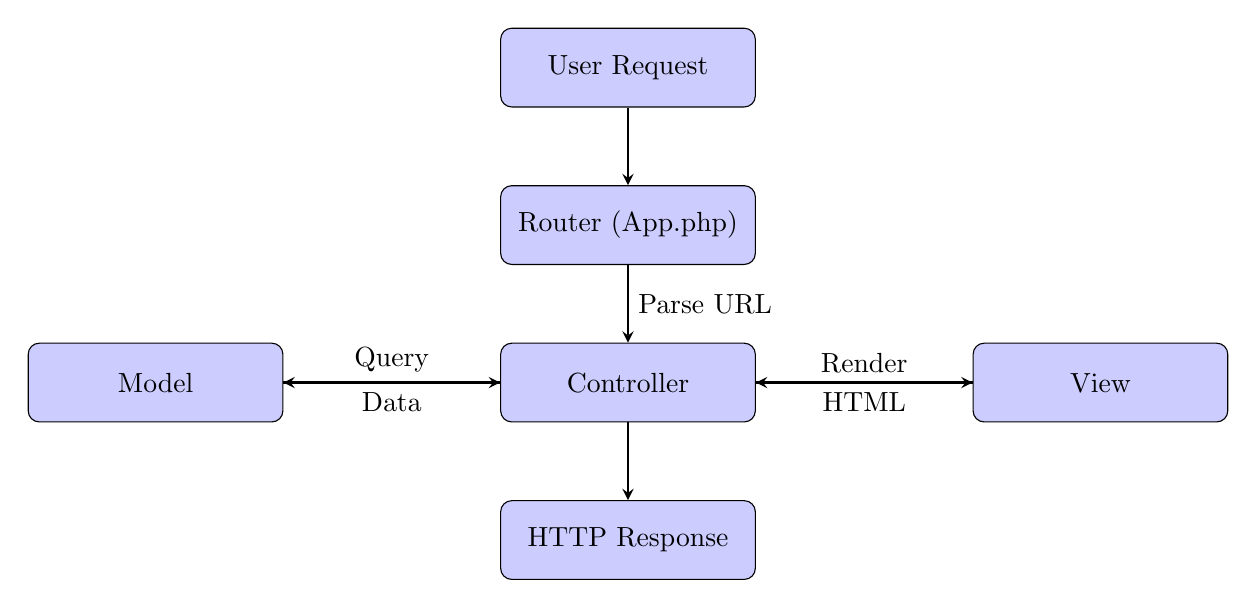
\begin{tikzpicture}[node distance=2cm, auto,
    box/.style={rectangle, draw, fill=blue!20, text width=3cm, text centered, rounded corners, minimum height=1cm},
    arrow/.style={->,>=stealth,thick}]

    \node[box] (user) {User Request};
    \node[box, below of=user] (router) {Router (App.php)};
    \node[box, below of=router] (controller) {Controller};
    \node[box, left of=controller, node distance=6cm] (model) {Model};
    \node[box, right of=controller, node distance=6cm] (view) {View};
    \node[box, below of=controller] (response) {HTTP Response};

    \draw[arrow] (user) -- (router);
    \draw[arrow] (router) -- node[right] {Parse URL} (controller);
    \draw[arrow] (controller) -- node[above] {Query} (model);
    \draw[arrow] (model) -- node[below] {Data} (controller);
    \draw[arrow] (controller) -- node[above] {Render} (view);
    \draw[arrow] (view) -- node[below] {HTML} (controller);
    \draw[arrow] (controller) -- (response);
\end{tikzpicture}
\caption{Luồng xử lý request trong mô hình MVC}
\label{fig:mvc-flow}
\end{figure}

\subsubsection{Các thành phần Core}

\textbf{1. Router - App.php:}
\begin{itemize}
    \item Parse URL thành: \texttt{[controller, method, params]}
    \item Load controller tương ứng
    \item Gọi method với parameters
    \item Xử lý 404 nếu không tìm thấy
\end{itemize}

\textbf{2. Base Controller - Controller.php:}
\begin{itemize}
    \item \texttt{model(\$name)}: Load model động
    \item \texttt{view(\$view, \$data)}: Render view với data
    \item \texttt{redirect(\$path)}: Chuyển hướng trang
    \item \texttt{isPost()}, \texttt{isGet()}: Kiểm tra HTTP method
\end{itemize}

\textbf{3. Database Wrapper - DB.php:}
\begin{itemize}
    \item PDO connection singleton
    \item \texttt{query(\$sql, \$params)}: Execute với prepared statements
    \item \texttt{single()}, \texttt{all()}: Fetch results
    \item Transaction support
\end{itemize}


% ------------------------------------------
\subsection{Cấu trúc thư mục}

Dự án được tổ chức theo cấu trúc MVC rõ ràng:

\begin{verbatim}
BTL_SachHay/
|-- app/                      # Application code
|   |-- config/               # Configuration files
|   |-- controllers/          # Controller classes
|   |-- core/                 # Core framework files
|   |-- models/               # Model classes
|   +-- views/                # View templates
|-- public/                   # Public assets
|   |-- index.php             # Entry point
|   |-- css/                  # Stylesheets
|   |-- js/                   # JavaScript files
|   +-- images/               # Images
+-- db/                       # Database files
\end{verbatim}


% ------------------------------------------
\subsection{Tính năng hệ thống}

\subsubsection{Khách (Guest)}

Người dùng chưa đăng nhập có thể:
\begin{itemize}
    \item Truy cập trang chủ và xem sản phẩm nổi bật
    \item Duyệt danh sách sản phẩm theo danh mục
    \item Xem chi tiết sản phẩm
    \item Tìm kiếm sản phẩm
    \item Đọc tin tức và bài viết
    \item Xem trang giới thiệu, hỏi đáp, liên hệ
    \item Đăng ký tài khoản mới
    \item Đăng nhập vào hệ thống
\end{itemize}

\subsubsection{Thành viên (Customer)}

Sau khi đăng nhập, thành viên có thêm các quyền:
\begin{itemize}
    \item Thêm sản phẩm vào giỏ hàng
    \item Quản lý giỏ hàng (tăng/giảm số lượng, xóa)
    \item Xem và chỉnh sửa thông tin cá nhân
    \item Xem lịch sử đơn hàng
    \item Quản lý danh sách sản phẩm yêu thích
    \item Nhận thông báo về đơn hàng
    \item Đăng xuất khỏi hệ thống
\end{itemize}

\subsubsection{Quản trị viên (Admin)}

Các tính năng quản trị:
\begin{itemize}
    \item Quản lý danh sách người dùng và phân quyền
    \item Thêm/sửa/xóa sản phẩm và danh mục
    \item Quản lý đơn hàng và trạng thái giao hàng
    \item Quản lý nội dung tin tức, Q\&A, liên hệ
    \item Cấu hình nội dung trang tĩnh
\end{itemize}

% ------------------------------------------
\subsection{Luồng hoạt động (Flowcharts)}

\textbf{Luồng đăng nhập:}
\begin{enumerate}
    \item Người dùng truy cập trang đăng nhập
    \item Nhập username và password
    \item Hệ thống kiểm tra thông tin
    \item Nếu đúng: Tạo session, redirect về trang chủ
    \item Nếu sai: Hiển thị thông báo lỗi
\end{enumerate}

\textbf{Luồng mua hàng:}
\begin{enumerate}
    \item Khách hàng duyệt sản phẩm
    \item Click "Thêm vào giỏ" trên sản phẩm mong muốn
    \item Kiểm tra đăng nhập - nếu chưa, yêu cầu đăng nhập
    \item Sản phẩm được thêm vào giỏ hàng (Session)
    \item Khách hàng có thể tiếp tục mua hoặc checkout
    \item Xem giỏ hàng, điều chỉnh số lượng
    \item Tiến hành thanh toán
    \item Xác nhận đơn hàng
\end{enumerate}
